In the previous sections we described ROMC from the user's
point-of-view; the demonstration focused on performing the inference
with the ready-to-use tools. Apart from this use-case, a practitioner
can also use ROMC as a meta-algorithm, adding custom algorithms as
part of the method. Our implementation allows such intervention. In
the rest of the chapter, We will initially present the main internal
classes and then then we will exhibit how to add custom methods.

\subsubsection{Entities presentation}

In figure \ref{fig:example_training} we provide an overview of the
classes used in the algorithm. The class $\pinline{ROMC}$ can be
thought as the interface between the user and the method. The rest of
the classes are responsible for the back-end functionality. It is
important for the reader to remember the sequence of the events for
performing the inference, as demonstrated in figure
\ref{fig:romc_overview}.

The class \pinline{ROMC} is the main class of the method; it is
initialised when the user calls the method for the first time and its
state is updated throughout the inference.The initialisation of the
\pinline{ROMC} object sets the attributes \pinline{model},
\pinline{model_prior}, \pinline{bounds}, \pinline{inference_state} to
the appropriate values; the rest of the attributes are set to
\pinline{None}.\footnote{in all cases, we use the value None for
  indicating that an attribute is not yet initialised."}.

The \pinline{_sample_nuisance()} routine samples $n_1$ integers from
the discrete integer distribution. The \pinline{_define_objectives()}
routine initialises $n_1$ \pinline{OptimisationProblem} objects,
appends them to a \pinline{List} and stores this \pinline{List} as the
\pinline{romc.optim_problems} attribute. The
\pinline{_define_objectives()} function, initialises the only the
attributes \pinline{objective} and \pinline{bounds} of the
\pinline{OptimisationProblem}; the rest are set to \pinline{None}. The
attribute \pinline{objective}, which is a \pinline{Callable}, is
created by setting the seed of the \pinline{model.generate()} to a
specific integer, turning the random generator to a deterministic.

Afterwards, depending on the boolean argument
\pinline{use_bo=True/False}, the function \pinline{_solve_gradients}
or \pinline{_solve_bo} is called. Both of them follow the same
sequence of steps; for each optimisation problem (a) they solve it and
(b) they initialise a \pinline{RomcOptimisationResult} object with the
solution and (c) they store it as the
\pinline{OptimisationProblem.result} attribute. Although they both
apply the same sequence of steps, each method uses a different
optimisation scheme; \pinline{_solve_gradients} uses the
\pinline{minimize} class of the \pinline{scipy.optimize} library
\autocite{2020SciPy-NMeth}, whereas \pinline{_solve_bo} uses the
\pinline{BoDeterministic} class.  \pinline{BoDeterministic} is a class
we implemented for performing Bayesian Optimisation and fitting a
Gaussian Process surrogate model to the objective function. It relies
on the Gpy framework \autocite{gpy2014} for fitting the Gaussian
Process. The only difference between \pinline{_solve_gradients} and
\pinline{_solve_bo}, as effect in the state of the
\pinline{OptimisationProblem} class, is the initialisation of the
attribute \pinline{OptimisationProblem.surrogate}, which is done only
by \pinline{_solve_bo}. The attribute is set to a \pinline{Callable}
that wraps the \pinline{GPyRegression.predict_mean} function. If
\pinline{_solve_gradients} is called, the attribute remains
\pinline{None}.

At this level, all optimisation problems have been solved. The method
\pinline{_filter_solutions} is used for discarding the optimisation
results that are over threshold. Afterwards, \pinline{_build_boxes}
estimates the bounding boxes around the accepted objective
functions. For each accepted objective function, a
\pinline{RegionConstructor} object is initialised in order to
construct the region. In the current implementation, for each
objective function we constract a single bounding box, but this may
change in a future approach; for being able to support multiple
bounding boxes per objective function, we decided to return a
\pinline{List} of \pinline{NDimBoundingBox} objects\footnote{Each
  \pinline{NDimBoundingBox} object represents a region.}. The
\pinline{List} is stored as the \pinline{OptimisationProblem.regions}
attribute.

By now, we have estimated the bounding boxes around the optimal
points. The last step, before defining the posterior, is the fitting
local surrogate models. This step is optional and is performend only
if the argument \pinline{fit_models} is set to \pinline{True}. The
routine \pinline{_fit_models}, fits a quadratic model on the area
around the optimal point for each objective function. For achieving
so, it asks for samples from the \pinline{NDimBoundingBox} object and
evaluates them using the \pinline{OptimisationProblem.objective}
function. Afterwards, based on these points, it fits a quadratic model
using the \pinline{linear_model.LinearRegression} and
\pinline{preprocessing.PolynomialFeatures} functions of the
\pinline{scikit-learn} package \autocite{scikit-learn}. The trained
model is stored as the attribute
\pinline{OptimisationProblem.local_surrogate}.


Finally, the \pinline{_define_posterior} method is used for creating
the \pinline{RomcPosterior} object and storing it as the
\pinline{ROMC.posterior} attribute. The method collects (a) all the
bounding boxes created so far (accessing the
\pinline{OptimisationProblem.regions} attributes and (b) all the objective functions. As the objective function it collects either \pinline{OptimisationProblem.local_surrogate} or \pinline{OptimisationProblem.surrogate} or \pinline{OptimisationProblem.objective}, depending on which one is available based on the previous steps.

The description above summarises the sequence of steps needed for the
training part of the method. The conclusion is that a \pinline{ROMC}
object is intialised when the user calls the method. Throughout the
inference process, the \pinline{ROMC} object is always as a specific state,
which gets updated whenever an algorithmic step is executed. The rest
of the classes provide objects which are stored as attributes of
\pinline{ROMC}.

\begin{figure}[h]
    \begin{center}
      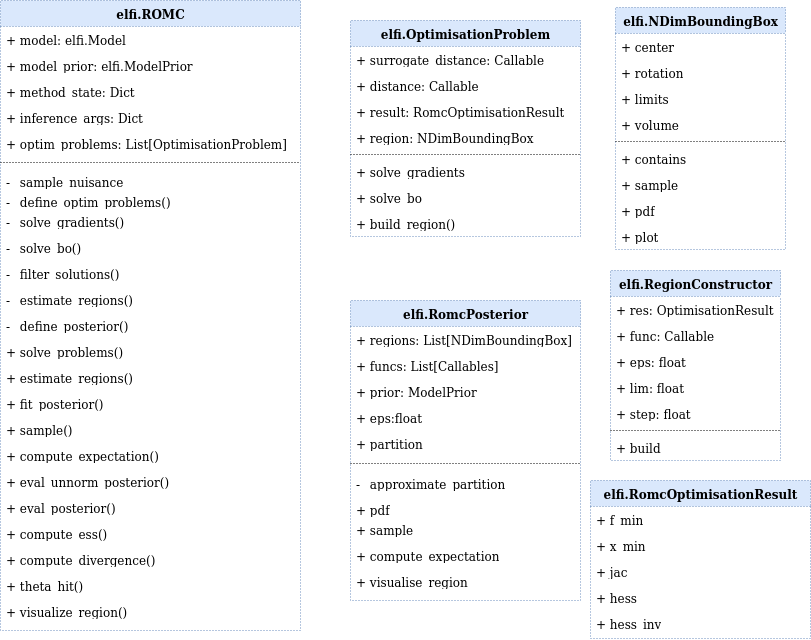
\includegraphics[width=\textwidth]{./Thesis/graphs/RomcEntityDiagram.png}
    \end{center}
  \caption{Histogram of distances and visualisation of a specific region.}
  \label{fig:example_training}
\end{figure}


\subsubsection{Extensibility of the ROMC method}

In this section we will explain how a practitioner may replace some
parts of the ROMC method with their custom alogorithms. We can locate
at least four such points; (a) the gradient-based solver (b) the
Bayesian Optimisation solver (c) the bounding box region construction
and (d) the fitting of the local surrogate models. Each of the
aforementioned tasks may be approached with completely different
algorithms than the ones we propose, without the rest of the method to
change.

The four replacable parts described above, are solved using the four
methods of the \pinline{OptimisatioProblem} class;
\pinline{solve_gradients(**kwargs)}, \pinline{solve_bo(**kwargs)},
\pinline{build_region(**kwargs)},
\pinline{fit_local_surrogate(**kwargs)}. Therefore, the practitioner
should not alter at all the basic \pinline{ROMC} class. Instead, they
should deploy a custom optimisation problem class which inherits the
basic \pinline{OptimisatioProblem} class and overwrites the above four
functiones with custom ones. The only rule that should be followed
carefully, is that the cutom methods must have the same effect on the
attributes of the \pinline{ROMC} class, i.e. update them with the
appropriate objects as presented in table \ref{tab:extensibility}. For
example, a function that replaces \pinline{solve_gradients()} must
have the effect of storing a \pinline{RomcOptimisationResult} object
to the \pinline{OptimisationObject} attribute.

\begin{center} \label{tab:extensibility} \captionof{table}{Table
    explaining the appropriate effect of each replacable routine,
    i.e. which object they should attach to the appropriate
    attribute. The functions of the first column (\pinline{ROMC}
    class) call the correpsonding functions of the second column
    (\pinline{OptimisationProblem} class). The functions of the second
    column should execute their main functionality and update the
    appropriate attribute with a certain object, as described in the
    third column. }


\begin{tabular}{ c|c }
\hline
\pinline{OptimisationProblem} & \pinline{Effect} \\
\hline \hline
\pinline{solve_gradients()} & \pinline{result <- RomcOptimisationResult} \\
\hline
\multirow{ 2}{*}{\pinline{solve_bo()}} & \pinline{result <- RomcOptimisationResult} \\
& \pinline{surrogate <- Callable} \\
\hline
\pinline{build_region()} & \pinline{regions <- List[NDimBoundingBox]}\\
\hline
\pinline{fit_local_surrogate()} & \pinline{local_surrogate <- Callable}\\
\hline
\end{tabular}
\end{center}

\subsubsection*{Example: use a Neural Network as a local surrogate model}

Let's say we have observed that the local area around $\theta_i^*$ is
too complex to be represented by a simple quadratic model\footnote{as
  in the current implementation}. Hence, the user selects a neural
network as a good alternative. In the following snippet, we
demonstrate how they could implement this enhancement, without much
effort; (a) they have to develop the neural network using the package
of their choice (b) they must create a custom optimisation class which
inherites the basic \pinline{OptimisationClass} and (c) they have to
overwrite the \pinline{fit_local_surrogate} routine, with one that
sets the neural network's prediction function as the
\pinline{local_surrograte} attribute. The argument \pinline{**kwargs}
may be used for passing all the important arguments e.g.\ training
epochs, gradient step etc. If, for example, they would like to set the
size of the training set dynamically, we may replace \pinline{x =
  self.regions[0].sample(30)} with \pinline{x =
  self.regions[0].sample(kwargs["nof_examples"])}. Finally, they must
pass the custom optimisation class, when calling the \pinline{ROMC}
method.

\begin{pythoncode}
  class NeuralNetwork:
      def __init__(self, **kwargs):
          # set the input arguments

      def train(x, y):
          # training code

      def predict(x):
          # prediction code

  # Inherit the base optimisation class
  class customOptim(elfi.methods.parameter_inference.OptimisationProblem):
      def __init__(self, **kwargs):
          super(customOptim, self).__init__(**kwargs)

      # overwrite the function you want to replace
      def fit_local_surrogate(**kwargs):
          # init and train the NN
          x = self.regions[0].sample(30) # 30 training points
          y = [np.array([self.objective(ii) for ii in x])]
          nn = NeuralNet()
          nn.train(x,y)

          # set the appropriate attribute
          self.local_surrogate = nn.predict

          # update the state
          self.state["local_surrogate"] = True

  # pass the custom inference method as argument
  romc = elfi.ROMC(dist, bounds, custom_optim_class=customOptim)
\end{pythoncode}
